\chapter{Experimental Results}\label{ch:expRes}

In the following chapter the different variants of the RLS and the (1+1) EA are now analysed empirically for the best algorithm depending on the input. Additionally for most lemmas from the previous chapters there are also tests if they actually hold in practice.

\section{Code}
The complete java code used for all empirical studies is available on GitHub:\newline
https://github.com/Err404NameNotFound/PartitionSolvingWithEAs.\newline
\subsection{The Algorithms}
All different variants of the RLS function more or the less the same. They start with an initial random value and then optimise this one value in the loop. The loop can be summarised like this:
\begin{enumerate}
      \item generate a number k of bits to be flipped (algorithm specific)
      \item flip k random bits
      \item evaluate fitness of the mutated individual
      \item replace old value with new value if new value is better
      \item repeat if not optimal
\end{enumerate}
The (1+1) EA variants behave differently on the first impression as there every bit is flipped independently with probability $c/n$. This can be seen as n independent Bernoulli trials with probability $c/n$. The amount of bits that are flipped is therefore binomial distributed and the algorithm can be implemented exactly as the versions of the RLS. The same holds for the pMut operator which generates a number k from a powerlaw distribution and then flips k bits. This leads to only one implementation of a partition solving algorithm which is not only given the input array of numbers but also a generator for the amount of bits to be flipped in each step. The random values for the amount of bits to be flipped are generated according to this table:

\begin{tabular}[h]{c c}
      Algorithm & Returned value                                                                          \\
      \hline
      RLS       & 1                                                                                       \\
      RLS-N(k)  & $y \in \{1,\dots,k\}$ with probability $\frac{\binom{n}{y}}{\sum_{i=1}^k \binom{n}{i}}$ \\
      RLS-R(k)  & uniform random value $y \in \{1,\dots,k\}$                                              \\
      (1+1) EA  & binomial distributed value from \textasciitilde$B(n,c/n)$                               \\
      pMut      & random value generated from powerlaw distribution with parameter $\beta$                \\
\end{tabular}



\begin{algorithm}[bt]
      \caption{\textsc{GenericPartitionSolver}}\label{alg:genericPartition}

      % Some settings
      \DontPrintSemicolon %dontprintsemicolon
      \SetFuncSty{textsc}

      % The algorithm
      \BlankLine
      choose x uniform random from ${\{0,1\}}^n$\;
      \While{$x$ not optimal}
      {
      $x' \leftarrow x$\;
      $k \leftarrow \text{kGenerator.generate()}$\;
      flip $k$ uniform random bits of $x'$\;
      {
      \If{$f(x') \le f(x)$}
      {
            $x \leftarrow x'$\;
      }
      }
      }
\end{algorithm}

\subsection{Random number generation}

Java only provides a random number generator for uniform distributed values for any integer interval or random double values $\in \left[0, 1\right)$. For this project this does not suffice as for an efficient way of implementing the (1+1) EA or simply for generating a binomial distributed input another random number generator is needed. One of the needed distributions is a binomial distribution. The simplest way to generate a number \textasciitilde$B(m,p)$ would be to run a loop $m$ times and add 1 to the generated number if a uniform random value $\in \left[0, 1\right)$ is less than $p$. This works perfectly fine and generates numbers according to the distribution. With low values for p this approach is rather inefficient and especially for values of $p=1/m$. The expected value in this case is 1 but generating a random number takes time $\mathcal{O}(m)$. Another more efficient way was implemented by StackOverflow user \href{https://stackoverflow.com/users/2166798/pjs}{pjs} on \href{https://stackoverflow.com/questions/23561551/a-efficient-binomial-random-number-generator-code-in-java}{stackoverflow} inspired by Devroyes method introduced in~\cite{devroye2006nonuniform}. This method has an expected running time of $\mathcal{O}(mp)$ which is equal to the expected value of the distribution. For the case of $p=1/m$ this runs in expected constant time in comparison to $\mathcal{O}(m)$ for the naive way. This number generation was also used for the implementation of the (1+1) EA instead of running a for loop in every step.

\begin{algorithm}[h]
      \caption{\textsc{Binomial random number generator}}\label{alg:binomialRNG}

      % Some settings
      \DontPrintSemicolon %dontprintsemicolon
      \SetFuncSty{textsc}
      $q \leftarrow \ln(1.0 - p)$\;
      $x \leftarrow 0$\;
      $sum \leftarrow 0$\;
      \While{true}
      {
      $sum \leftarrow sum +\ln(\text{random()}) / (n - x)$\; \tcp{random() generates a random value $\in \left[0, 1\right)$}
      \If{sum < q}
      {
            return $x$\;
      }
      $x \leftarrow x + 1$\;
      }
\end{algorithm}

The next generator needed is for exponentially distributed values. This generator is only necessary for the generation of exponentially distributed inputs but not for the algorithms itself. The easiest way to generate exponentially distributed values is the naive way: generating a uniform random value until the generated value is at least as big as the probability. The expected running time of this algorithm is equal to the expected value of the distribution $1/p$. So this method is comparably effective to the approach used for binomial random number generation.

\begin{algorithm}[h]
      \caption{\textsc{Exponential random number generator}}\label{alg:exponentialRNG}

      % Some settings
      \DontPrintSemicolon %dontprintsemicolon
      \SetFuncSty{textsc}
      $sum \leftarrow 0$\; \tcp{random() generates a random value $\in \left[0, 1\right)$}
      \While{\text{random()} < q}
      {
            $sum \leftarrow sum+1$\;
      }
      return $sum$\;
\end{algorithm}

The last generator needed is for powerlaw distributed values. This generator is in contrast to the exponential number generator only needed for the algorithm with the $pmut_\beta$ mutation operator. This implementation is also from stackoverflow. The user \href{https://stackoverflow.com/users/52738/gnovice}{gnovice} provided the following formula on \href{https://stackoverflow.com/questions/918736/random-number-generator-that-produces-a-power-law-distribution}{this} page on stackoverflow:
\[
      x = {[(b^{n+1} - q^{n+1})*y + a^{n+1}]}^{1/(n+1)}
\]
$a$ is the lower bound, $b$ the upper bound, $n$ the parameter of the distribution and $y$ the number generated uniform random $\in \left[0, 1\right)$. The idea behind the formula and the formula itself is explained in a \href{https://mathworld.wolfram.com/RandomNumber.html}{mathworld} page.


\section{Do inputs have perfect partitions?}
\subsection{Binomial Inputs}

Lemma~\ref{lemma:BinomialSolvable} is only valid for larger n. In practice the bound is much smaller depending on the expected value of a single value. Another factor deciding how likely an input is to have a perfect partition is if n is even or odd. To determine the influence of both factors two experiments were conducted. The goal of the first experiment was to determine the influence of the array size to the input having a perfect partition and the fact if n is even or odd. So for every possible combination of $p \in \{0.1, 0.2, \dots , 0.8, 0.9\}, m \in \{10,100,1000,10^4,10^5\} \text{ and } n \in \{2,3,4,\dots,19,20\}$ 1000 randomly generated inputs of size $n$ were tested for a perfect partition. Due to the small values for $n$ it was possible to brute force the results in a short amount of time. The results are visualised in figure~\ref{fig:firstBinPercentage} to figure~\ref{fig:lastBinPercentage}.
On the x-axis is the size of the input and on the y-axis the percentage of inputs that had a perfect partition. The different graphs in each figure resemble the different values of p used for generating the inputs. The graph for 0.1 resembles the percentage of inputs that had a perfect partition with values generated from the distribution \textasciitilde$B(m,0.1)$ with $m$ being dependent on the figure. For figure~\ref{fig:firstBinPercentage} $m$ has the value 10.\newline
It is easy to see that for small inputs sizes it is relevant if n is even or odd for higher expected values as all curves in figure~\ref{fig:lastBinPercentage} oscillate between 0\% and 100\% for $n\ge14$. For uneven inputs the probability of a perfect partition decreases much more drastically with m as for even inputs because the expected value of a single number increases with m. If all values are much higher the small differences between the values can no longer even out the fact of one set has more elements than the other. The oscillation therefore increases with increasing m. For $n=20$ all 1000 inputs had a perfect partition for every combination of $p$ and $m$ but for $n=19$ only combinations where $mp\le300$ holds lead to at least one out of 1000 having a perfect partition. For expected values of up to $10^5$ it seems to be almost granted that an input of length 20 has a perfect partition if it is binomial distributed.
Even for only 12 binomial generated values more than 50\% of the inputs had a perfect partition (see figure~\ref{fig:lastBinPercentage}). Another visible effect is the decreasing percentage with rising p. This may be a direct result of the value chosen for p but can also be an indirect result as the value for p changes the expected value for a constant m. The expected value may have an influence on the number of perfect partitions because it influences the highest value of the input.
For uniform distributed inputs Borgs showed that the coefficient of \#bits needed to encode the max value/$n$ has a huge impact on the number of perfect partitions~\cite{borgs2001phase}. For a coefficient < 1 the probability of a perfect partition tends to 1 and for a coefficient > 1 it tends to 0. This was only proven for the uniform distributed input, but it might also hold for a binomial distributed input. This leads to the second experiment.

\begin{figure}[h]
      \centering
      \begin{minipage}[b]{0.45\textwidth}
            \caption{Percentage of Binomial inputs with perfect partitions for m = 10}
            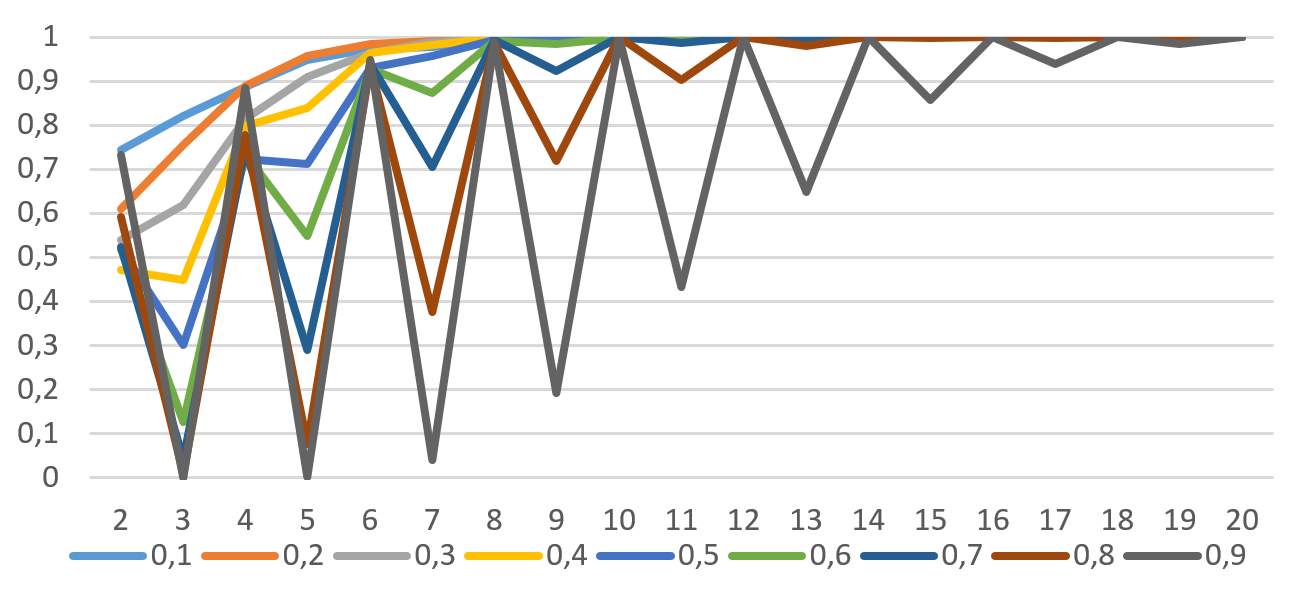
\includegraphics[width=\textwidth]{figures/images/solvabilityOfInputs/binomial_Input_Solvable_m10.png}\label{fig:firstBinPercentage}
      \end{minipage}
      \hspace{0.75cm}
      \begin{minipage}[b]{0.45\textwidth}
            \caption{Percentage of Binomial inputs with perfect partitions for m = 100}
            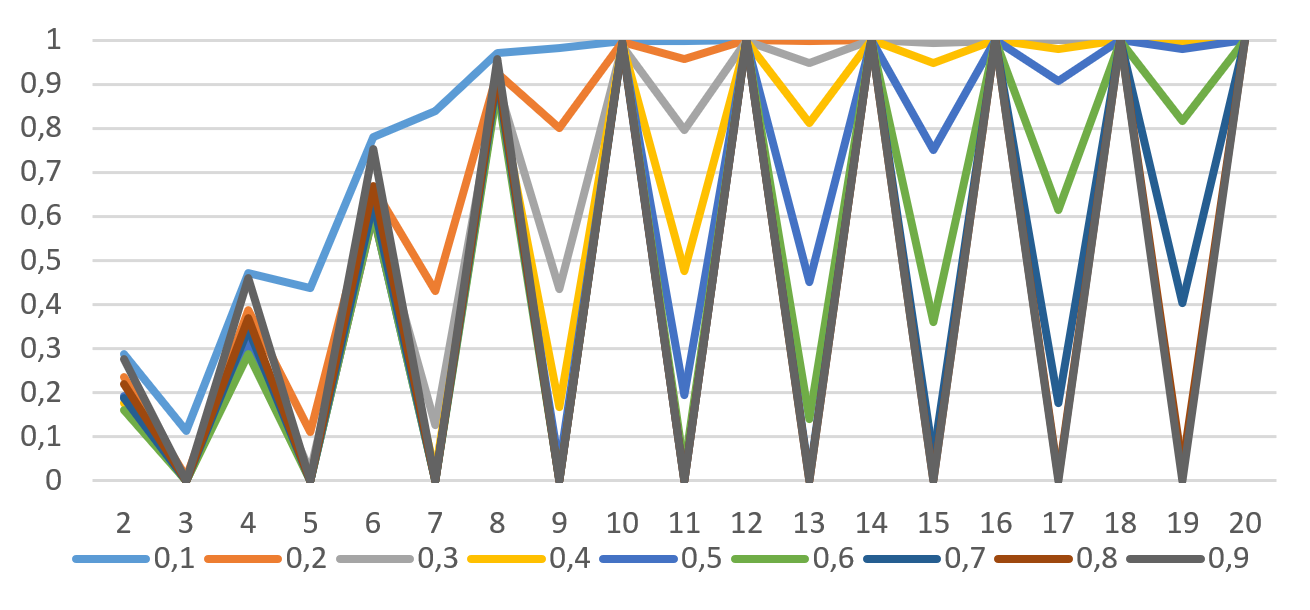
\includegraphics[width=\textwidth]{figures/images/solvabilityOfInputs/binomial_Input_Solvable_m100.png}
      \end{minipage}
\end{figure}

\begin{figure}[h]
      \centering
      \begin{minipage}[b]{0.45\textwidth}
            \caption{Percentage of Binomial inputs with perfect partitions for m = 1000}
            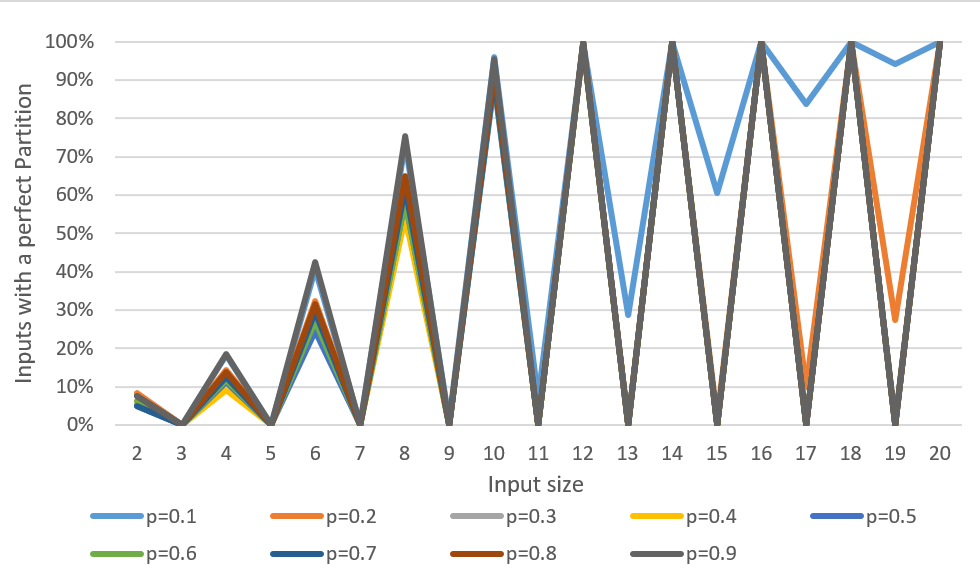
\includegraphics[width=\textwidth]{figures/images/solvabilityOfInputs/binomial_Input_Solvable_m1000.png}
      \end{minipage}
      \hspace{0.75cm}
      \begin{minipage}[b]{0.45\textwidth}
            \caption{Percentage of Binomial inputs with perfect partitions for m = 10000}
            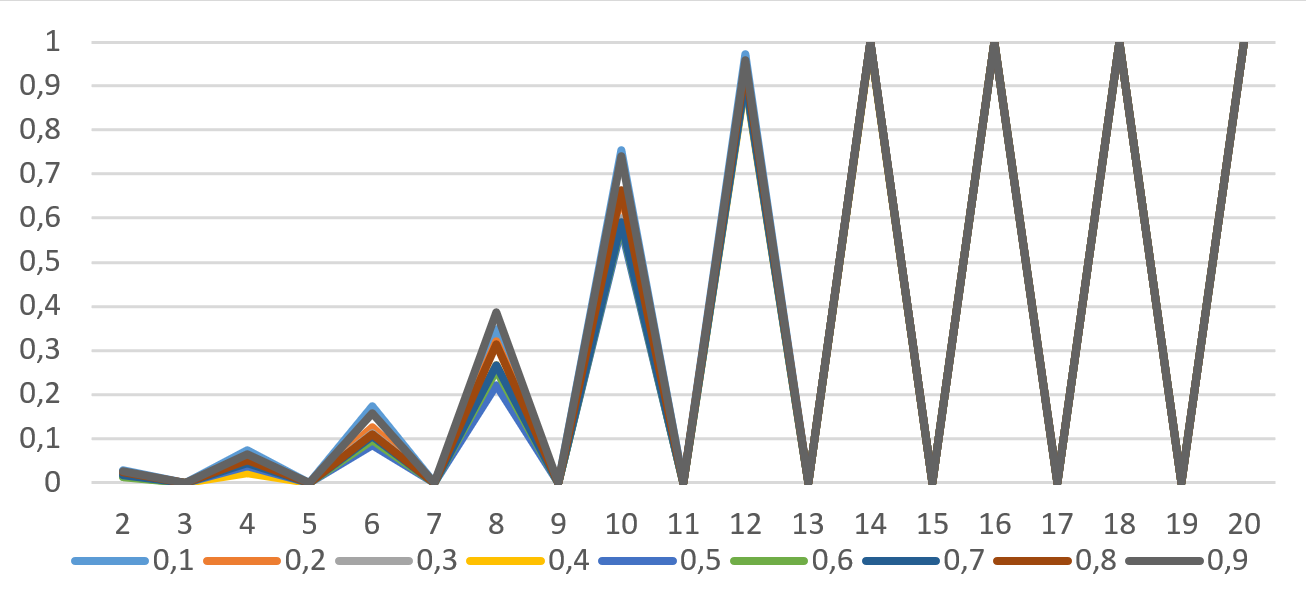
\includegraphics[width=\textwidth]{figures/images/solvabilityOfInputs/binomial_Input_Solvable_m10000.png}
      \end{minipage}
\end{figure}

\begin{figure}[h]
      \caption{Percentage of Binomial inputs with perfect partitions for m = 100000}
      \centering
      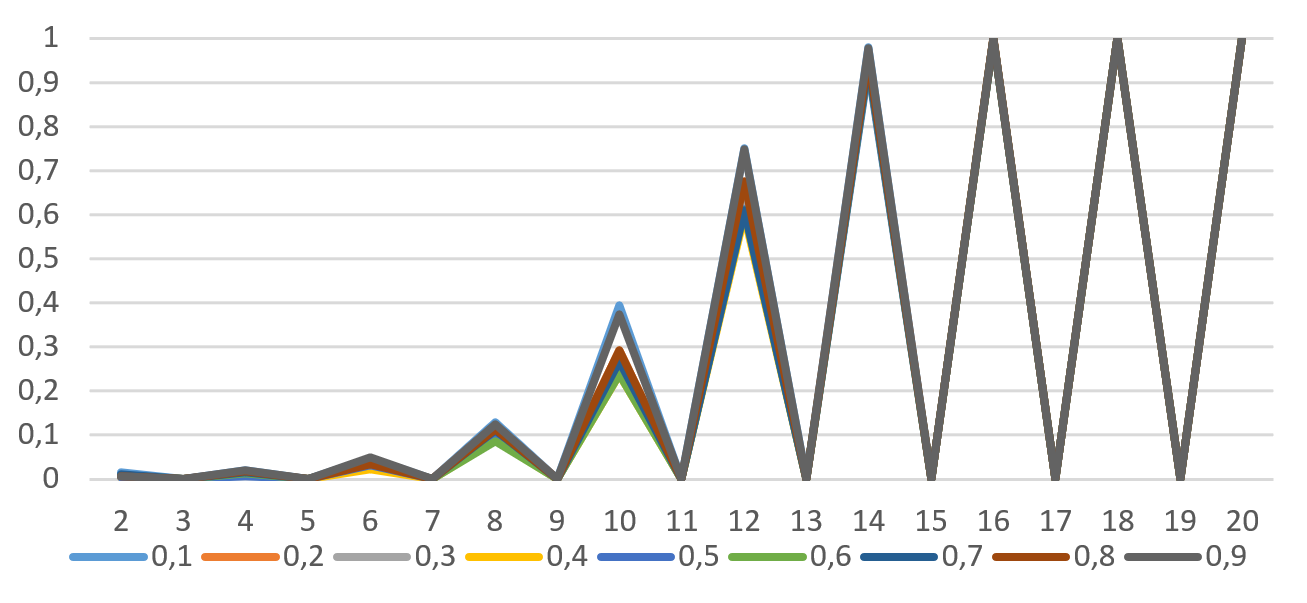
\includegraphics[width=0.45\textwidth]{figures/images/solvabilityOfInputs/binomial_Input_Solvable_m100000.png}\label{fig:lastBinPercentage}
\end{figure}


In the second experiment the inputs were generated a bit differently. Here the goal was to keep the expected value fixed for any combination of $p$ and $n$ and set the value of $m$ to $e/p$ for all $e \in \{10, 20, 30, 40, 50, 100, 200, 500, 1000, 2000, 5000, 10000, 50000\}$ so that $E(X)=mp=e/p\cdot p=e$. With this setup the influence of the expected value is almost isolated from the other parameters. The probability is still linked to $p$ as $p$ also influences the variance $mp(1-p)$. By looking at figure~\ref{fig:firstBinPercentage2} to figure~\ref{fig:lastBinPercentage2} it seems as if the value of $p$ has a much smaller influence than the expected value. For a fixed expected value and a fixed input size a higher value for $p$ seems to only slightly increase the percentage of inputs with a perfect partition. The expected value influences the percentage significantly more. For $p=0.1, n=14$ the value decreases from 100\% at $E(X)=10$ to below 20\% at $E(X)=50000$. For $p=0.9$ the percentage only drops below 50\% but still decreases by a factor of 2.

\begin{figure}[h]
      \centering
      \begin{minipage}[b]{0.45\textwidth}
            \caption{Percentage of Binomial inputs with perfect partitions for p = 0.1}
            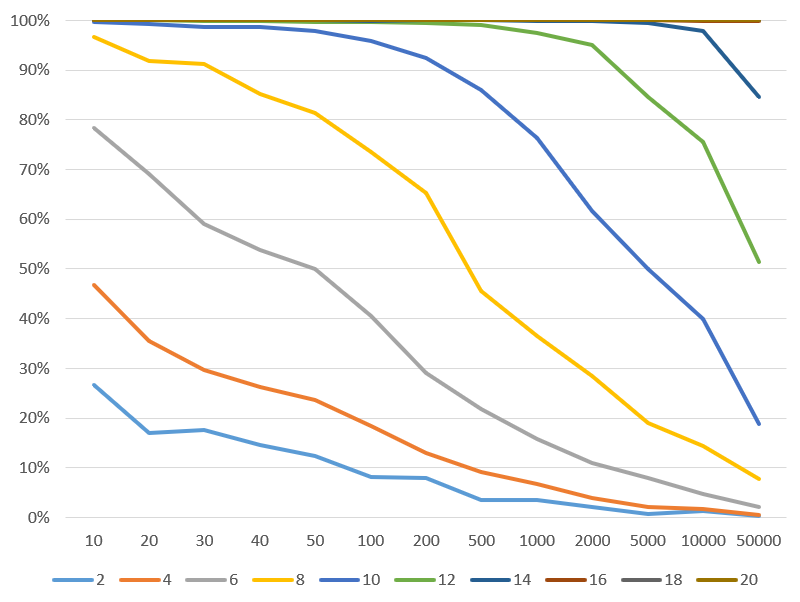
\includegraphics[width=\textwidth]{figures/images/solvabilityOfInputs/solvability0_1.png}\label{fig:firstBinPercentage2}
      \end{minipage}
      \hspace{0.75cm}
      \begin{minipage}[b]{0.45\textwidth}
            \caption{Percentage of Binomial inputs with perfect partitions for p = 0.2}
            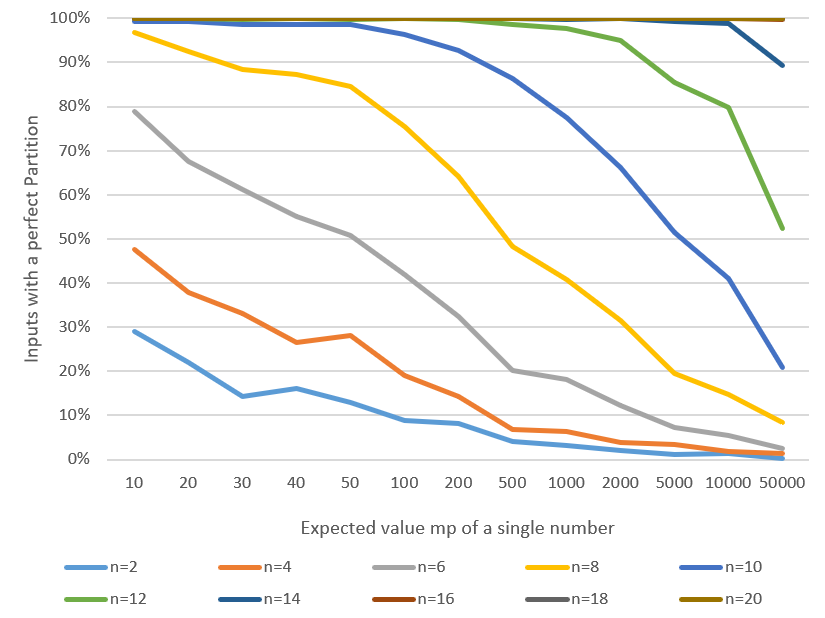
\includegraphics[width=\textwidth]{figures/images/solvabilityOfInputs/solvability0_2.png}
      \end{minipage}
\end{figure}


\begin{figure}[h]
      \centering
      \begin{minipage}[b]{0.45\textwidth}
            \caption{Percentage of Binomial inputs with perfect partitions for p = 0.3}
            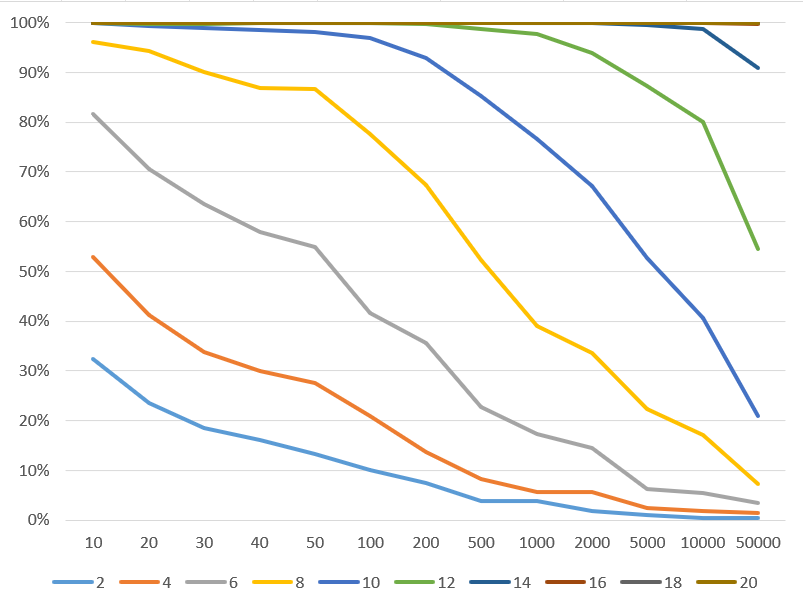
\includegraphics[width=\textwidth]{figures/images/solvabilityOfInputs/solvability0_3.png}
      \end{minipage}
      \hspace{0.75cm}
      \begin{minipage}[b]{0.45\textwidth}
            \caption{Percentage of Binomial inputs with perfect partitions for p = 0.4}
            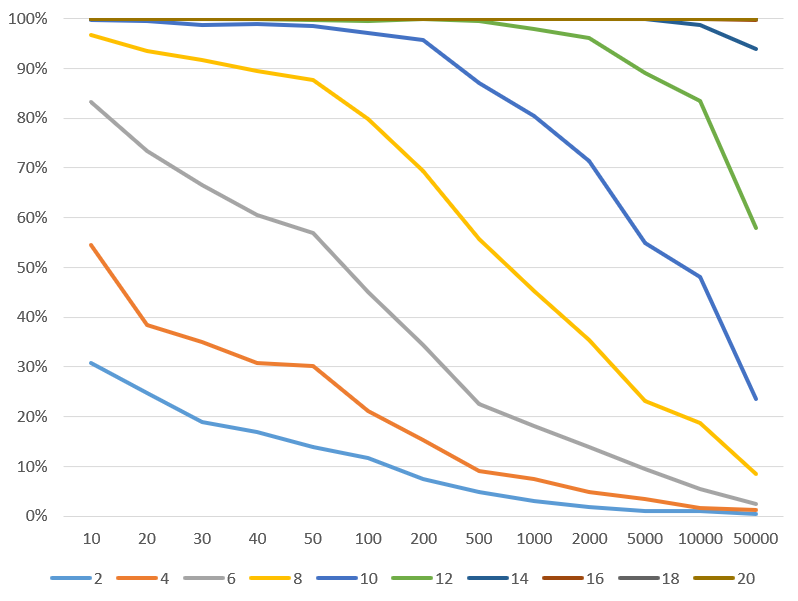
\includegraphics[width=\textwidth]{figures/images/solvabilityOfInputs/solvability0_4.png}
      \end{minipage}
\end{figure}


\begin{figure}[h]
      \centering
      \begin{minipage}[b]{0.45\textwidth}
            \caption{Percentage of Binomial inputs with perfect partitions for p = 0.5}
            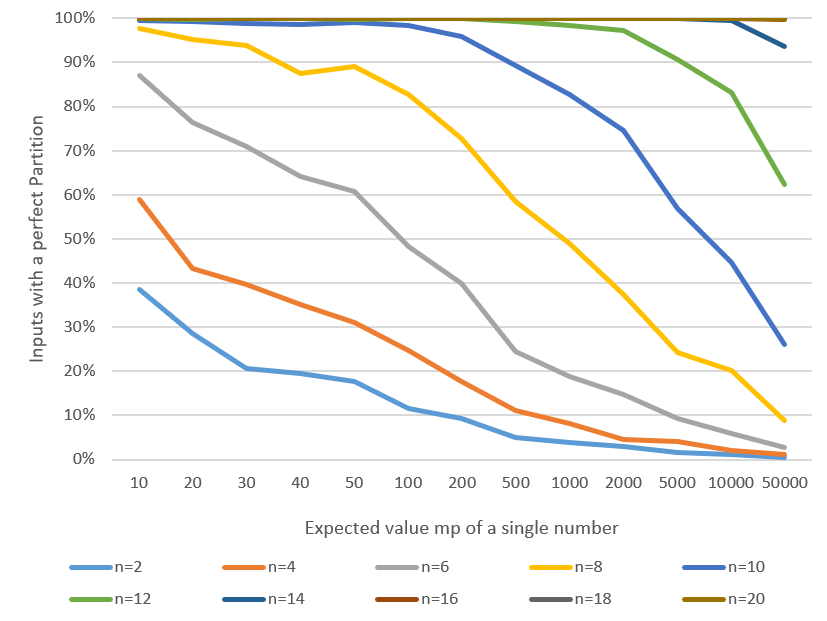
\includegraphics[width=\textwidth]{figures/images/solvabilityOfInputs/solvability0_5.png}
      \end{minipage}
      \hspace{0.75cm}
      \begin{minipage}[b]{0.45\textwidth}
            \caption{Percentage of Binomial inputs with perfect partitions for p = 0.9}
            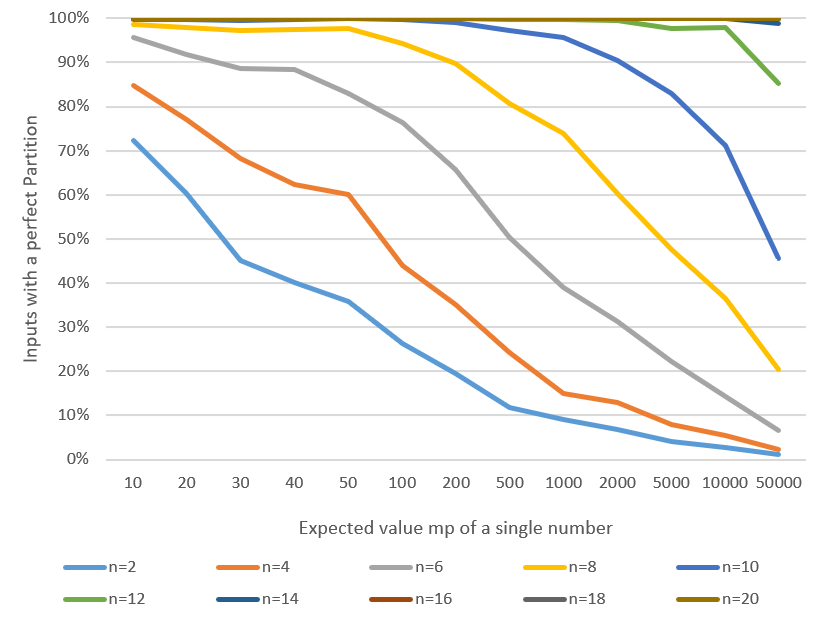
\includegraphics[width=\textwidth]{figures/images/solvabilityOfInputs/solvability0_9.png}\label{fig:lastBinPercentage2}
      \end{minipage}
\end{figure}

The last experiment showed that for $n=20$ 1000/1000 inputs had a perfect partition. This raised the question of how the amount of perfect partition changes with changing values for $m, p, n$.

% \section{Binomial distributed inputs}
% \subsection{RLS Comparison}

% \begin{tabular}[h]{cccccccc}
%       algo type       & RLS-N & RLS-N & RLS-R & RLS-R & RLS-R & RLS-N   & RLS     \\
%       algo param      & k=2   & k=4   & k=2   & k=4   & k=3   & k=3     & -       \\
%       avg mut/change  & 2,000 & 4,000 & 1,603 & 2,553 & 2,000 & 2,728   & 1,000   \\
%       avg mut/step    & 2,000 & 4,000 & 1,500 & 2,500 & 1,999 & 3,000   & 1,000   \\
%       \hline
%       total avg count & 318   & 434   & 499   & 579   & 681   & 518.428 & 920.109 \\
%       avg eval count  & 318   & 434   & 499   & 579   & 681   & 395.440 & 50      \\
%       max eval count  & 1.648 & 3.243 & 3.094 & 3.737 & 4.717 & 917.134 & 50      \\
%       min eval count  & 20    & 28    & 11    & 17    & 16    & 0       & 50      \\
%       \hline
%       fails           & 0     & 0     & 0     & 0     & 0     & 234     & 999     \\
%       fail ratio      & 0,000 & 0,000 & 0,000 & 0,000 & 0,000 & 0,234   & 0,999   \\
%       avg fail dif    & -1    & -1    & -1    & -1    & -1    & 1       & 254     \\
% \end{tabular}

% \subsection{(1+1) EA Comparison}
% \subsection{pmut Comparison}
% \subsection{Comparison of the best variants}

% \section{Uniform distributed inputs}
% \subsection{RLS Comparison}
% \subsection{(1+1) EA Comparison}
% \subsection{pmut Comparison}
% \subsection{Comparison of the best variants}

% \section{Exponential distributed inputs}
% \subsection{RLS Comparison}
% \subsection{(1+1) EA Comparison}
% \subsection{pmut Comparison}
% \subsection{Comparison of the best variants}

% \section{OneMax Equivalent for PARTITION}
% This kind of input is more or less equivalent to the OneMax problem. All values except the last are either 1 or uniform
% random in any interval. The last value is the sum of all other values. The optimal solution is therefore the 000\dots01 or
% the 111\dots01 string. So the best solution is almost identical to OneMax. In the previous chapter the $\mathcal{O}(nlogn)$ bound was
% proven for the (1+1) EA and the RLS. This seems to hold in practice:
% TODO: insert Graph showing RLS and (1+1) EA need time O(nlogn)

% For OneMax the mutation rate of 1/n is proven to be optimal for the (1+1) EA (TODO insert cite). This seems to be also
% true for the equivalent for PARTITION. For Both the (1+1) EA and both new Variants of the RLS
% \subsection{RLS Comparison}

% \subsection{(1+1) EA Comparison}
% \subsection{pmut Comparison}
% \subsection{Comparison of the best variants}

% \section{Carsten Witts worst case input}
% \subsection{RLS Comparison}
% \subsection{(1+1) EA Comparison}
% \subsection{pmut Comparison}
% \subsection{Comparison of the best variants}

% \section{PowerLawDistributed}
% \subsection{RLS Comparison}
% \subsection{(1+1) EA Comparison}
% \subsection{pmut Comparison}
% \subsection{Comparison of the best variants}

% \section{Multiple distributions overlapped}
% \subsection{RLS Comparison}
% \subsection{(1+1) EA Comparison}
% \subsection{pmut Comparison}
% \subsection{Comparison of the best variants}

% \section{Multiple distributions mixed}
% \subsection{RLS Comparison}
% \subsection{(1+1) EA Comparison}
% \subsection{pmut Comparison}
% \subsection{Comparison of the best variants}

% \section{Multiple distributions mixed \& overlapped}
% \subsection{RLS Comparison}
% \subsection{(1+1) EA Comparison}
% \subsection{pmut Comparison}
% \subsection{Comparison of the best variants}

% BEGIN RESULTS

\section{Binomial distributed values}
\subsection{RLS Comparison}
\begin{tabular}[h]{cccccccc}
algo type&          RLS-N&   RLS-N&   RLS-R&   RLS-R&   RLS-R&   RLS-N&     RLS\\
algo param&           k=2&     k=4&     k=2&     k=4&     k=3&     k=3&       -\\
avg mut/change&     2,000&   4,000&   1,603&   2,553&   2,000&   2,728&   1,000\\
avg mut/step&       2,000&   4,000&   1,500&   2,500&   1,999&   3,000&   1,000\\
\hline
total avg count&      318&     434&     499&     579&     681& 518.428& 920.109\\
avg eval count&       318&     434&     499&     579&     681& 395.440&      50\\
max eval count&     1.648&   3.243&   3.094&   3.737&   4.717& 917.134&      50\\
min eval count&        20&      28&      11&      17&      16&       0&      50\\
\hline
fails&                  0&       0&       0&       0&       0&     234&     999\\
fail ratio&         0,000&   0,000&   0,000&   0,000&   0,000&   0,234&   0,999\\
avg fail dif&          -1&      -1&      -1&      -1&      -1&       1&     254\\
\end{tabular}
\subsection{(1+1) EA Comparison}
\begin{tabular}[h]{ccccccccc}
algo type&          EA-SM&   EA-SM&   EA-SM&   EA-SM&      EA&   EA-SM&   EA-SM&   EA-SM\\
algo param&           3/n&     4/n&     2/n&     5/n&       -&    10/n&    50/n&   100/n\\
avg mut/change&     3,101&   3,968&   2,343&   4,859&   1,698&   9,732&  49,544&  99,494\\
avg mut/step&       2,999&   4,003&   2,002&   4,999&   1,001&   9,998&  49,998&  99,997\\
\hline
total avg count&      646&     701&     706&     857&   1.123&   1.508&   8.175&  15.485\\
avg eval count&       646&     701&     706&     857&   1.123&   1.508&   8.175&  15.485\\
max eval count&     5.346&   5.692&   3.415&   5.572&   7.001&  12.112&  52.831& 145.269\\
min eval count&        23&       4&      30&       9&      23&      14&      27&      69\\
\hline
fails&                  0&       0&       0&       0&       0&       0&       0&       0\\
fail ratio&         0,000&   0,000&   0,000&   0,000&   0,000&   0,000&   0,000&   0,000\\
avg fail dif&          -1&      -1&      -1&      -1&      -1&      -1&      -1&      -1\\
\end{tabular}
\subsection{pmut Comparison}
\begin{tabular}[h]{cccccccccc}
algo type&           pmut&    pmut&    pmut&    pmut&    pmut&    pmut&    pmut&    pmut&    pmut\\
algo param&         -2,25&   -2,00&   -1,75&   -2,50&   -2,75&   -3,00&   -3,25&   -1,50&   -1,25\\
avg mut/change&     3,822&   6,266&  14,371&   2,804&   2,347&   1,995&   1,843&  38,318&  92,365\\
avg mut/step&       4,344&   8,504&  22,176&   2,878&   2,272&   1,933&   1,732&  70,476& 224,535\\
\hline
total avg count&      652&     668&     675&     688&     697&     718&     758&     785&   1.050\\
avg eval count&       652&     668&     675&     688&     697&     718&     758&     785&   1.050\\
max eval count&     4.340&   4.506&   5.616&   5.098&   9.140&   5.081&   6.189&   6.542&   7.837\\
min eval count&        14&       4&       9&      12&      27&      10&      11&      21&       7\\
\hline
fails&                  0&       0&       0&       0&       0&       0&       0&       0&       0\\
fail ratio&         0,000&   0,000&   0,000&   0,000&   0,000&   0,000&   0,000&   0,000&   0,000\\
avg fail dif&          -1&      -1&      -1&      -1&      -1&      -1&      -1&      -1&      -1\\
\end{tabular}
\subsection{Comparison of the best variants}
\begin{tabular}[h]{cccc}
algo type&        RLS-N& EA-SM&  pmut\\
algo param&         k=2&   3/n& -2,25\\
avg mut/change&   2,000& 3,092& 3,965\\
avg mut/step&     2,000& 2,999& 4,339\\
\hline
total avg count&    302&   677&   691\\
avg eval count&     302&   677&   691\\
max eval count&   1.610& 6.404& 5.205\\
min eval count&       9&    33&    17\\
\hline
fails&                0&     0&     0\\
fail ratio&       0,000& 0,000& 0,000\\
avg fail dif&        -1&    -1&    -1\\
\end{tabular}
\section{Exponential distributed values}
\subsection{RLS Comparison}
\begin{tabular}[h]{cccccccc}
algo type&         RLS-R&  RLS-R&  RLS-R&  RLS-N&  RLS-N&  RLS-N&    RLS\\
algo param&          k=2&    k=3&    k=4&    k=2&    k=3&    k=4&      -\\
avg mut/change&    1,477&  1,959&  2,431&  2,000&  3,000&  4,000&  1,000\\
avg mut/step&      1,500&  2,001&  2,501&  2,000&  3,000&  4,000&  1,000\\
\hline
total avg count&   2.592&  2.945&  3.259&  3.497&  4.463&  5.345&  6.650\\
avg eval count&    2.592&  2.945&  3.259&  3.497&  4.463&  5.345&  2.055\\
max eval count&   19.845& 23.932& 28.532& 23.824& 30.881& 41.600& 25.889\\
min eval count&        8&     22&     19&     18&     43&     19&     23\\
\hline
fails&                 0&      0&      0&      0&      0&      0&      5\\
fail ratio&        0,000&  0,000&  0,000&  0,000&  0,000&  0,000&  0,005\\
avg fail dif&         -1&     -1&     -1&     -1&     -1&     -1&      1\\
\end{tabular}
\subsection{(1+1) EA Comparison}
\begin{tabular}[h]{ccccccccc}
algo type&          EA-SM&      EA&   EA-SM&   EA-SM&   EA-SM&   EA-SM&   EA-SM&   EA-SM\\
algo param&           2/n&       -&     3/n&     4/n&     5/n&    10/n&    50/n&   100/n\\
avg mut/change&     2,255&   1,554&   3,038&   3,948&   4,883&   9,821&  49,798&  99,814\\
avg mut/step&       2,000&   1,000&   3,000&   4,001&   5,000&   9,999&  49,998& 100,001\\
\hline
total avg count&    3.712&   3.833&   4.195&   4.472&   5.465&   8.282&  21.648&  29.404\\
avg eval count&     3.712&   3.833&   4.195&   4.472&   5.465&   8.282&  21.648&  29.404\\
max eval count&    39.593&  53.450&  33.598&  42.449&  55.717&  65.522& 149.048& 281.857\\
min eval count&        18&      13&      15&      14&      25&      23&      46&      17\\
\hline
fails&                  0&       0&       0&       0&       0&       0&       0&       0\\
fail ratio&         0,000&   0,000&   0,000&   0,000&   0,000&   0,000&   0,000&   0,000\\
avg fail dif&          -1&      -1&      -1&      -1&      -1&      -1&      -1&      -1\\
\end{tabular}
\subsection{pmut Comparison}
\begin{tabular}[h]{cccccccccc}
algo type&           pmut&    pmut&    pmut&    pmut&    pmut&    pmut&    pmut&    pmut&    pmut\\
algo param&         -3,25&   -3,00&   -2,50&   -2,75&   -2,25&   -2,00&   -1,75&   -1,50&   -1,25\\
avg mut/change&     1,682&   1,872&   2,688&   2,150&   3,704&   6,938&  16,352&  41,906& 107,789\\
avg mut/step&       1,730&   1,936&   2,918&   2,267&   4,355&   8,463&  22,369&  70,989& 225,029\\
\hline
total avg count&    2.575&   2.732&   2.734&   2.776&   2.809&   3.165&   3.486&   4.389&   6.151\\
avg eval count&     2.575&   2.732&   2.734&   2.776&   2.809&   3.165&   3.486&   4.389&   6.151\\
max eval count&    73.911&  34.215&  75.791&  42.620&  25.352&  31.966&  37.725&  50.454&  55.022\\
min eval count&        33&      17&      11&       0&      35&       9&       5&      23&      19\\
\hline
fails&                  0&       0&       0&       0&       0&       0&       0&       0&       0\\
fail ratio&         0,000&   0,000&   0,000&   0,000&   0,000&   0,000&   0,000&   0,000&   0,000\\
avg fail dif&          -1&      -1&      -1&      -1&      -1&      -1&      -1&      -1&      -1\\
\end{tabular}
\subsection{Comparison of the best variants}
\begin{tabular}[h]{cccc}
algo type&         RLS-R&   pmut&  EA-SM\\
algo param&          k=2&  -3,25&    2/n\\
avg mut/change&    1,483&  1,693&  2,258\\
avg mut/step&      1,500&  1,729&  2,001\\
\hline
total avg count&   2.407&  2.695&  3.421\\
avg eval count&    2.407&  2.695&  3.421\\
max eval count&   23.155& 57.661& 52.762\\
min eval count&       19&     11&     19\\
\hline
fails&                 0&      0&      0\\
fail ratio&        0,000&  0,000&  0,000\\
avg fail dif&         -1&     -1&     -1\\
\end{tabular}
\section{Uniform distributed inputs}
\subsection{RLS Comparison}
\begin{tabular}[h]{cccccccc}
algo type&            RLS-N&     RLS-R&     RLS-R&     RLS-N&     RLS-R&     RLS-N&       RLS\\
algo param&             n=2&       r=3&       r=4&       n=3&       r=2&       n=4&         -\\
avg mut/change&       2,000&     1,996&     2,476&     3,000&     1,502&     4,000&     1,000\\
avg mut/step&         2,000&     2,000&     2,500&     3,000&     1,500&     4,000&     1,000\\
\hline
total avg count&     83.118&   104.748&   105.513&   112.223&   114.486&   121.927& 2.443.567\\
avg eval count&      83.118&   104.748&   105.513&   112.223&   114.486&   121.927&    45.834\\
max eval count&     778.110& 1.453.252&   898.974& 1.377.471&   915.268&   816.633&   485.275\\
min eval count&         197&       126&        45&       212&       271&       155&       128\\
\hline
fails&                    0&         0&         0&         0&         0&         0&       447\\
fail ratio&           0,000&     0,000&     0,000&     0,000&     0,000&     0,000&     0,447\\
avg fail dif&            -1&        -1&        -1&        -1&        -1&        -1&         1\\
\end{tabular}
\subsection{(1+1) EA Comparison}
\begin{tabular}[h]{ccccccc}
algo type&            EA-SM&     EA-SM&     EA-SM&     EA-SM&     EA-SM&        EA\\
algo param&             3/n&       2/n&       4/n&       5/n&      10/n&         -\\
avg mut/change&       3,102&     2,287&     4,014&     4,937&     9,924&     1,577\\
avg mut/step&         3,000&     2,000&     4,000&     5,000&    10,000&     1,000\\
\hline
total avg count&    122.098&   122.690&   124.634&   132.509&   183.213&   213.186\\
avg eval count&     122.098&   122.690&   124.634&   132.509&   183.213&   213.186\\
max eval count&     956.375&   920.658& 1.128.158& 1.457.069& 1.298.089& 2.509.163\\
min eval count&         174&       188&       265&       384&         6&       111\\
\hline
fails&                    0&         0&         0&         0&         0&         0\\
fail ratio&           0,000&     0,000&     0,000&     0,000&     0,000&     0,000\\
avg fail dif&            -1&        -1&        -1&        -1&        -1&        -1\\
\end{tabular}
\subsection{pmut Comparison}
\begin{tabular}[h]{cccccccccc}
algo type&             pmut&      pmut&      pmut&      pmut&      pmut&      pmut&      pmut&      pmut&      pmut\\
algo param&           -2,25&     -2,00&     -3,00&     -2,75&     -2,50&     -1,75&     -1,50&     -3,25&     -1,25\\
avg mut/change&       3,898&     5,603&     1,891&     2,259&     2,720&    28,035&    94,745&     1,724&   334,887\\
avg mut/step&         4,568&    10,031&     1,933&     2,274&     2,933&    34,684&   158,937&     1,728&   718,814\\
\hline
total avg count&    111.048&   115.812&   121.406&   122.184&   123.348&   149.182&   157.279&   157.451&   199.763\\
avg eval count&     111.048&   115.812&   121.406&   122.184&   123.348&   149.182&   157.279&   157.451&   199.763\\
max eval count&     854.290&   487.327&   773.065&   736.059&   695.178& 1.079.073& 1.927.473&   795.211& 1.243.407\\
min eval count&         375&       746&     1.502&     3.103&       896&     4.047&       360&     1.516&       775\\
\hline
fails&                    0&         0&         0&         0&         0&         0&         0&         0&         0\\
fail ratio&           0,000&     0,000&     0,000&     0,000&     0,000&     0,000&     0,000&     0,000&     0,000\\
avg fail dif&            -1&        -1&        -1&        -1&        -1&        -1&        -1&        -1&        -1\\
\end{tabular}
\subsection{Comparison of the best variants}
\begin{tabular}[h]{cccc}
algo type&            RLS-N&     EA-SM&      pmut\\
algo param&             n=2&       3/n&     -2,25\\
avg mut/change&       2,000&     3,109&     4,273\\
avg mut/step&         2,000&     3,000&     4,555\\
\hline
total avg count&     84.884&   116.576&   124.046\\
avg eval count&      84.884&   116.576&   124.046\\
max eval count&     741.833& 1.176.762& 1.159.541\\
min eval count&          52&       178&       178\\
\hline
fails&                    0&         0&         0\\
fail ratio&           0,000&     0,000&     0,000\\
avg fail dif&            -1&        -1&        -1\\
\end{tabular}
\section{OneMax Equivalent for PARTITION}
\subsection{RLS Comparison}
\begin{tabular}[h]{cccccccc}
algo type&            RLS&   RLS-R&   RLS-R&   RLS-R&   RLS-N&   RLS-N&   RLS-N\\
algo param&             -&     k=2&     k=3&     k=4&     k=2&     k=3&     k=4\\
avg mut/change&     1,000&   1,181&   1,688&   1,865&     NaN&     NaN&     NaN\\
avg mut/step&       1,000&   1,500&   2,000&   2,500&     NaN&     NaN&     NaN\\
\hline
total avg count&   90.931& 168.311& 236.317& 307.533& 921.030& 921.030& 921.030\\
avg eval count&    90.931& 168.311& 236.317& 307.533&      -1&      -1&      -1\\
max eval count&   156.854& 296.206& 498.474& 595.831&       0&       0&       0\\
min eval count&    64.941& 120.582& 158.304& 212.193&      -1&      -1&      -1\\
\hline
fails&                  0&       0&       0&       0&   1.000&   1.000&   1.000\\
fail ratio&         0,000&   0,000&   0,000&   0,000&   1,000&   1,000&   1,000\\
avg fail dif&          -1&      -1&      -1&      -1&      53&      36&     263\\
\end{tabular}
\subsection{(1+1) EA Comparison}
\begin{tabular}[h]{ccccccccc}
algo type&             EA&   EA-SM&   EA-SM&   EA-SM&   EA-SM&   EA-SM&   EA-SM&   EA-SM\\
algo param&             -&     2/n&     3/n&     4/n&     5/n&    10/n&    50/n&   100/n\\
avg mut/change&     1,273&   1,750&   2,334&   2,965&     NaN&     NaN&     NaN&     NaN\\
avg mut/step&       1,000&   2,000&   3,000&   4,000&     NaN&     NaN&     NaN&     NaN\\
\hline
total avg count&  230.328& 297.602& 495.951& 860.736& 921.030& 921.030& 921.030& 921.030\\
avg eval count&   230.328& 297.602& 495.951& 812.983&      -1&      -1&      -1&      -1\\
max eval count&   399.393& 625.976& 839.325& 917.029&       0&       0&       0&       0\\
min eval count&   162.400& 193.796& 347.185& 635.812&      -1&      -1&      -1&      -1\\
\hline
fails&                  0&       0&       0&      99&     224&     224&     224&     224\\
fail ratio&         0,000&   0,000&   0,000&   0,442&   1,000&   1,000&   1,000&   1,000\\
avg fail dif&          -1&      -1&      -1&       1&      18&     570&   2.488&   3.115\\
\end{tabular}
\subsection{pmut Comparison}
\begin{tabular}[h]{cccccccccc}
algo type&           pmut&    pmut&    pmut&    pmut&    pmut&    pmut&    pmut&    pmut&    pmut\\
algo param&         -3,25&   -3,00&   -2,75&   -2,50&   -2,25&   -2,00&   -1,75&   -1,50&   -1,25\\
avg mut/change&     1,289&   1,359&   1,459&   1,591&   1,813&   2,207&   2,760&   3,604&   5,382\\
avg mut/step&       1,731&   1,934&   2,270&   2,907&   4,371&   8,486&  22,299&  70,692& 224,466\\
\hline
total avg count&  145.095& 149.664& 170.912& 181.099& 214.361& 249.102& 301.566& 415.413& 715.219\\
avg eval count&   145.095& 149.664& 170.912& 181.099& 214.361& 249.102& 301.566& 415.413& 683.204\\
max eval count&   217.932& 223.561& 254.330& 246.635& 365.378& 376.768& 431.629& 735.214& 853.181\\
min eval count&   111.061& 119.931& 120.965& 130.174& 161.244& 180.570& 232.166& 311.979& 492.686\\
\hline
fails&                  0&       0&       0&       0&       0&       0&       0&       0&       7\\
fail ratio&         0,000&   0,000&   0,000&   0,000&   0,000&   0,000&   0,000&   0,000&   0,135\\
avg fail dif&          -1&      -1&      -1&      -1&      -1&      -1&      -1&      -1&       1\\
\end{tabular}
\subsection{Comparison of the best variants}
\begin{tabular}[h]{cccc}
algo type&            RLS&    pmut&      EA\\
algo param&             -&   -3,25&       -\\
avg mut/change&     1,000&   1,287&   1,272\\
avg mut/step&       1,000&   1,729&   1,000\\
\hline
total avg count&   91.171& 143.121& 231.082\\
avg eval count&    91.171& 143.121& 231.082\\
max eval count&   153.143& 227.737& 446.942\\
min eval count&    65.783&  93.602& 165.818\\
\hline
fails&                  0&       0&       0\\
fail ratio&         0,000&   0,000&   0,000\\
avg fail dif&          -1&      -1&      -1\\
\end{tabular}
\section{Carsten Witts worst case input}
\subsection{RLS Comparison}
\begin{tabular}[h]{cccccccc}
algo type&         RLS-N&  RLS-R&  RLS-R&  RLS-R&  RLS-N&    RLS&  RLS-N\\
algo param&          k=3&    k=4&    k=3&    k=2&    k=4&      -&    k=2\\
avg mut/change&    3,000&  2,379&  1,985&  1,327&  3,997&  1,000&  1,998\\
avg mut/step&      3,000&  2,500&  2,000&  1,500&  4,000&  1,000&  2,000\\
\hline
total avg count&   1.436&  1.641&  1.905&  2.856&  4.420&  6.507&  6.693\\
avg eval count&    1.436&  1.641&  1.905&  2.856&  4.420&  3.755&  6.693\\
max eval count&   12.521& 15.338& 22.394& 26.297& 42.702& 31.837& 74.281\\
min eval count&        0&      0&      0&      0&      0&      0&      0\\
\hline
fails&                 0&      0&      0&      0&      0&      3&      0\\
fail ratio&        0,000&  0,000&  0,000&  0,000&  0,000&  0,003&  0,000\\
avg fail dif&         -1&     -1&     -1&     -1&     -1&  4.249&     -1\\
\end{tabular}
\subsection{(1+1) EA Comparison}
\begin{tabular}[h]{ccccccccc}
algo type&         EA-SM&  EA-SM&  EA-SM&  EA-SM&  EA-SM&  EA-SM&  EA-SM&     EA\\
algo param&        100/n&   50/n&   10/n&    5/n&    4/n&    3/n&    2/n&      -\\
avg mut/change&   99,982& 49,983& 10,028&  5,085&  4,112&  3,150&  2,244&  1,470\\
avg mut/step&     99,980& 49,975& 10,002&  5,001&  4,001&  3,000&  2,001&  1,000\\
\hline
total avg count&      73&     97&    397&    839&    966&  1.391&  1.827&  3.732\\
avg eval count&       73&     97&    397&    839&    966&  1.391&  1.827&  3.732\\
max eval count&      488&    736&  5.075&  8.348&  9.734& 14.546& 22.186& 44.370\\
min eval count&        0&      0&      0&      0&      0&      0&      0&      0\\
\hline
fails&                 0&      0&      0&      0&      0&      0&      0&      0\\
fail ratio&        0,000&  0,000&  0,000&  0,000&  0,000&  0,000&  0,000&  0,000\\
avg fail dif&         -1&     -1&     -1&     -1&     -1&     -1&     -1&     -1\\
\end{tabular}
\subsection{pmut Comparison}
\begin{tabular}[h]{cccccccccc}
algo type&           pmut&    pmut&    pmut&    pmut&    pmut&    pmut&    pmut&    pmut&    pmut\\
algo param&         -1,25&   -1,50&   -1,75&   -2,00&   -2,25&   -2,50&   -2,75&   -3,00&   -3,25\\
avg mut/change&   197,675&  69,384&  23,211&   8,999&   4,259&   2,819&   2,133&   1,802&   1,598\\
avg mut/step&     226,848&  69,933&  22,429&   8,747&   4,313&   2,911&   2,268&   1,934&   1,725\\
\hline
total avg count&       41&      85&     222&     536&     922&   1.368&   1.723&   2.080&   2.339\\
avg eval count&        41&      85&     222&     536&     922&   1.368&   1.723&   2.080&   2.339\\
max eval count&       226&     682&   2.033&   4.760&   9.749&  16.271&  18.953&  18.794&  25.383\\
min eval count&         0&       0&       0&       0&       0&       0&       0&       0&       0\\
\hline
fails&                  0&       0&       0&       0&       0&       0&       0&       0&       0\\
fail ratio&         0,000&   0,000&   0,000&   0,000&   0,000&   0,000&   0,000&   0,000&   0,000\\
avg fail dif&          -1&      -1&      -1&      -1&      -1&      -1&      -1&      -1&      -1\\
\end{tabular}
\subsection{Comparison of the best variants}
\begin{tabular}[h]{cccc}
algo type&           pmut&   EA-SM&   RLS-N\\
algo param&         -1,25&   100/n&     k=3\\
avg mut/change&   208,477&  99,891&   3,000\\
avg mut/step&     228,998& 100,014&   3,000\\
\hline
total avg count&       42&      68&   1.216\\
avg eval count&        42&      68&   1.216\\
max eval count&       231&     466&  13.896\\
min eval count&         0&       0&       0\\
\hline
fails&                  0&       0&       0\\
fail ratio&         0,000&   0,000&   0,000\\
avg fail dif&          -1&      -1&      -1\\
\end{tabular}
\section{Multiple distributions overlapped}
\subsection{RLS Comparison}
\begin{tabular}[h]{cccccccc}
algo type&           RLS-R&    RLS-R&    RLS-R&    RLS-N&    RLS-N&      RLS&    RLS-N\\
algo param&            r=4&      r=3&      r=2&      n=3&      n=2&        -&      n=4\\
avg mut/change&      2,413&    1,951&    1,478&    2,000&    1,000&    1,000&    3,000\\
avg mut/step&        2,503&    2,000&    1,500&    2,000&    1,000&    1,000&    3,000\\
\hline
total avg count&       539&      546&      608&      612&      729&      733&      930\\
avg eval count&        539&      546&      608&      612&      729&      733&      930\\
max eval count&      1.579&    1.661&    1.883&    2.629&    2.623&    2.371&    4.591\\
min eval count&         15&        8&       42&       53&       80&       59&       73\\
\hline
fails&                   0&        0&        0&        0&        0&        0&        0\\
fail ratio&          0,000&    0,000&    0,000&    0,000&    0,000&    0,000&    0,000\\
avg fail dif&           -1&       -1&       -1&       -1&       -1&       -1&       -1\\
\end{tabular}
\subsection{(1+1) EA Comparison}
\begin{tabular}[h]{ccccccc}
algo type&             EA-SM&      EA-SM&      EA-SM&         EA&      EA-SM&      EA-SM\\
algo param&              3/n&        2/n&        4/n&          -&        5/n&       10/n\\
avg mut/change&        3,009&      2,230&      3,863&      1,545&      4,762&      9,548\\
avg mut/step&          3,000&      2,000&      3,998&      0,999&      4,998&     10,000\\
\hline
total avg count&         599&        617&        701&        942&        968&     11.682\\
avg eval count&          599&        617&        701&        942&        968&     11.682\\
max eval count&        1.927&      1.769&      2.016&      3.284&      3.537&     63.180\\
min eval count&           56&         65&         85&         91&         51&        112\\
\hline
fails&                     0&          0&          0&          0&          0&          0\\
fail ratio&            0,000&      0,000&      0,000&      0,000&      0,000&      0,000\\
avg fail dif&             -1&         -1&         -1&         -1&         -1&         -1\\
\end{tabular}
\subsection{pmut Comparison}
\begin{tabular}[h]{cccccccccc}
algo type&             pmut&      pmut&      pmut&      pmut&      pmut&      pmut&      pmut&      pmut&      pmut\\
algo param&           -1,75&     -2,00&     -2,25&     -1,50&     -2,50&     -2,75&     -3,00&     -3,25&     -1,25\\
avg mut/change&      29,356&     9,267&     3,910&   123,650&     2,761&     2,150&     1,855&     1,673&   399,522\\
avg mut/step&        40,906&    10,981&     4,619&   226,724&     2,950&     2,256&     1,935&     1,729&  1192,167\\
\hline
total avg count&        454&       479&       501&       504&       515&       541&       555&       572&       722\\
avg eval count&         454&       479&       501&       504&       515&       541&       555&       572&       722\\
max eval count&       1.404&     1.423&     1.437&     1.606&     1.988&     1.434&     1.444&     1.800&     2.223\\
min eval count&          38&        19&        45&        47&        18&        18&        58&        27&        48\\
\hline
fails&                    0&         0&         0&         0&         0&         0&         0&         0&         0\\
fail ratio&           0,000&     0,000&     0,000&     0,000&     0,000&     0,000&     0,000&     0,000&     0,000\\
avg fail dif&            -1&        -1&        -1&        -1&        -1&        -1&        -1&        -1&        -1\\
\end{tabular}
\subsection{Comparison of the best variants}
\begin{tabular}[h]{cccc}
algo type&            pmut&    RLS-R&    EA-SM\\
algo param&          -1,75&      r=4&      3/n\\
avg mut/change&     30,999&    2,415&    3,015\\
avg mut/step&       42,499&    2,501&    3,002\\
\hline
total avg count&       463&      543&      586\\
avg eval count&        463&      543&      586\\
max eval count&      1.330&    1.613&    1.389\\
min eval count&         61&       50&       99\\
\hline
fails&                   0&        0&        0\\
fail ratio&          0,000&    0,000&    0,000\\
avg fail dif&           -1&       -1&       -1\\
\end{tabular}
\section{Multiple distributions mixed}
\subsection{RLS Comparison}
\begin{tabular}[h]{cccccccc}
algo type&               RLS-N&        RLS-R&        RLS-R&        RLS-R&        RLS-N&        RLS-N&          RLS\\
algo param&                n=3&          r=4&          r=3&          r=2&          n=4&          n=2&            -\\
avg mut/change&          2,000&        2,556&        2,059&        1,593&        3,000&          NaN&          NaN\\
avg mut/step&            2,000&        2,501&        2,000&        1,500&        3,000&          NaN&          NaN\\
\hline
total avg count&       125.951&      249.157&      265.643&      268.552&      307.558&    9.210.300&    9.210.300\\
avg eval count&        125.951&      249.157&      265.643&      268.552&      307.558&           -1&           -1\\
max eval count&        862.008&    1.939.594&    2.389.907&    2.012.463&    2.203.167&           -1&           -1\\
min eval count&            155&          276&          331&          267&          156&           -1&           -1\\
\hline
fails&                       0&            0&            0&            0&            0&        1.000&        1.000\\
fail ratio&              0,000&        0,000&        0,000&        0,000&        0,000&        1,000&        1,000\\
avg fail dif&               -1&           -1&           -1&           -1&           -1&          778&          785\\
\end{tabular}
\subsection{(1+1) EA Comparison}
\begin{tabular}[h]{ccccccc}
algo type&               EA-SM&        EA-SM&        EA-SM&        EA-SM&        EA-SM&           EA\\
algo param&                4/n&          3/n&          5/n&          2/n&         10/n&            -\\
avg mut/change&          3,981&        3,153&        4,887&        2,359&        9,759&        1,701\\
avg mut/step&            4,000&        3,000&        5,000&        2,000&       10,000&        1,000\\
\hline
total avg count&       244.704&      253.722&      268.529&      304.147&      346.669&      577.955\\
avg eval count&        244.704&      253.722&      268.529&      304.147&      346.669&      577.955\\
max eval count&      2.209.416&    2.340.925&    2.589.980&    2.416.509&    2.474.967&    3.776.445\\
min eval count&            269&          405&           24&          177&          236&           89\\
\hline
fails&                       0&            0&            0&            0&            0&            0\\
fail ratio&              0,000&        0,000&        0,000&        0,000&        0,000&        0,000\\
avg fail dif&               -1&           -1&           -1&           -1&           -1&           -1\\
\end{tabular}
\subsection{pmut Comparison}
\begin{tabular}[h]{cccccccccc}
algo type&                pmut&         pmut&         pmut&         pmut&         pmut&         pmut&         pmut&         pmut&         pmut\\
algo param&              -2,00&        -2,25&        -1,75&        -2,50&        -2,75&        -1,50&        -3,00&        -3,25&        -1,25\\
avg mut/change&          6,738&        4,132&       14,905&        2,817&        2,298&       37,736&        2,008&        1,832&       96,985\\
avg mut/step&            8,485&        4,364&       22,232&        2,906&        2,271&       70,714&        1,934&        1,729&      224,557\\
\hline
total avg count&       292.521&      292.763&      304.924&      307.403&      322.391&      337.925&      356.686&      377.068&      419.335\\
avg eval count&        292.521&      292.763&      304.924&      307.403&      322.391&      337.925&      356.686&      377.068&      419.335\\
max eval count&      3.811.952&    1.930.058&    2.875.275&    2.364.678&    2.233.600&    4.824.371&    2.832.218&    3.395.371&    3.133.351\\
min eval count&            535&          251&          202&          105&          124&          560&          104&           52&          841\\
\hline
fails&                       0&            0&            0&            0&            0&            0&            0&            0&            0\\
fail ratio&              0,000&        0,000&        0,000&        0,000&        0,000&        0,000&        0,000&        0,000&        0,000\\
avg fail dif&               -1&           -1&           -1&           -1&           -1&           -1&           -1&           -1&           -1\\
\end{tabular}
\subsection{Comparison of the best variants}
\begin{tabular}[h]{cccc}
algo type&               RLS-N&        EA-SM&         pmut\\
algo param&                n=3&          4/n&        -2,00\\
avg mut/change&          2,000&        3,996&        7,729\\
avg mut/step&            2,000&        4,000&        8,477\\
\hline
total avg count&       129.281&      267.444&      311.741\\
avg eval count&        129.281&      267.444&      311.741\\
max eval count&      1.276.682&    1.958.436&    2.465.518\\
min eval count&             62&          385&          245\\
\hline
fails&                       0&            0&            0\\
fail ratio&              0,000&        0,000&        0,000\\
avg fail dif&               -1&           -1&           -1\\
\end{tabular}
\section{Multiple distributions mixed \& overlapped}
\subsection{RLS Comparison}
\begin{tabular}[h]{cccccccc}
algo type&            RLS-N&     RLS-R&     RLS-R&     RLS-R&       RLS&     RLS-N&     RLS-N\\
algo param&             n=3&       r=3&       r=2&       r=4&         -&       n=2&       n=4\\
avg mut/change&       2,000&     1,903&     1,468&     2,321&     1,000&     1,000&     3,000\\
avg mut/step&         2,000&     2,001&     1,500&     2,500&     1,000&     1,000&     3,000\\
\hline
total avg count&      1.193&     1.326&     1.348&     1.406&     1.776&     1.780&     1.850\\
avg eval count&       1.193&     1.326&     1.348&     1.406&     1.776&     1.780&     1.850\\
max eval count&       3.692&     3.666&     3.490&     3.833&     4.568&     4.700&     5.159\\
min eval count&          44&        65&        94&        33&       109&        55&       102\\
\hline
fails&                    0&         0&         0&         0&         0&         0&         0\\
fail ratio&           0,000&     0,000&     0,000&     0,000&     0,000&     0,000&     0,000\\
avg fail dif&            -1&        -1&        -1&        -1&        -1&        -1&        -1\\
\end{tabular}
\subsection{(1+1) EA Comparison}
\begin{tabular}[h]{ccccccc}
algo type&             EA-SM&      EA-SM&      EA-SM&         EA&      EA-SM&      EA-SM\\
algo param&              3/n&        2/n&        4/n&          -&        5/n&       10/n\\
avg mut/change&        2,883&      2,146&      3,698&      1,514&      4,583&      9,553\\
avg mut/step&          3,000&      2,002&      4,000&      1,001&      5,001&     10,000\\
\hline
total avg count&       1.577&      1.648&      1.938&      2.224&      2.579&     22.183\\
avg eval count&        1.577&      1.648&      1.938&      2.224&      2.579&     22.183\\
max eval count&        4.466&      4.510&      5.481&      6.566&      8.345&     93.948\\
min eval count&           66&        169&        159&        232&        179&        225\\
\hline
fails&                     0&          0&          0&          0&          0&          0\\
fail ratio&            0,000&      0,000&      0,000&      0,000&      0,000&      0,000\\
avg fail dif&             -1&         -1&         -1&         -1&         -1&         -1\\
\end{tabular}
\subsection{pmut Comparison}
\begin{tabular}[h]{cccccccccc}
algo type&             pmut&      pmut&      pmut&      pmut&      pmut&      pmut&      pmut&      pmut&      pmut\\
algo param&           -2,50&     -2,25&     -2,75&     -2,00&     -3,25&     -3,00&     -1,75&     -1,50&     -1,25\\
avg mut/change&       2,500&     3,777&     2,053&     7,773&     1,622&     1,785&    22,640&    97,028&   310,342\\
avg mut/step&         2,914&     4,680&     2,271&    10,908&     1,733&     1,928&    41,606&   222,441&  1196,549\\
\hline
total avg count&      1.368&     1.395&     1.418&     1.422&     1.423&     1.428&     1.554&     1.797&     2.493\\
avg eval count&       1.368&     1.395&     1.418&     1.422&     1.423&     1.428&     1.554&     1.797&     2.493\\
max eval count&       4.195&     4.235&     4.599&     4.348&     4.609&     4.040&     4.775&     5.609&     8.303\\
min eval count&         133&        90&        49&        23&        95&        99&        94&       134&        87\\
\hline
fails&                    0&         0&         0&         0&         0&         0&         0&         0&         0\\
fail ratio&           0,000&     0,000&     0,000&     0,000&     0,000&     0,000&     0,000&     0,000&     0,000\\
avg fail dif&            -1&        -1&        -1&        -1&        -1&        -1&        -1&        -1&        -1\\
\end{tabular}
\subsection{Comparison of the best variants}
\begin{tabular}[h]{cccc}
algo type&            RLS-N&      pmut&     EA-SM\\
algo param&             n=3&     -2,50&       3/n\\
avg mut/change&       2,000&     2,875&     2,882\\
avg mut/step&         2,000&     2,972&     3,000\\
\hline
total avg count&      1.225&     1.424&     1.579\\
avg eval count&       1.225&     1.424&     1.579\\
max eval count&       3.347&     3.791&     4.611\\
min eval count&          50&       139&       103\\
\hline
fails&                    0&         0&         0\\
fail ratio&           0,000&     0,000&     0,000\\
avg fail dif&            -1&        -1&        -1\\
\end{tabular}